\pc{2}{28/10}

\question List five non-proprietary Internet applications and the application-layer protocols that they use.

\question For a P2P file-sharing application, do you agree with the following statement?
\begin{center}
    \emph{``There is no notion of client and server sides of a communication session.''}
\end{center}
Why or why not?

\question What information is used by a process running on one host to identify a process running on another host?

\question Suppose you wanted to do a transaction from a remote client to a server as fast as possible. Would you use UDP or TCP? Why?

\question What is meant by a handshaking protocol?

\question For the client-server application over TCP shown in Figure \ref{fig:prac-2-1}, why must the server program be executed before the client program? 
For a similar client-server application over UDP, why may the client program be executed before the server program?

\begin{figure}
    \centering
    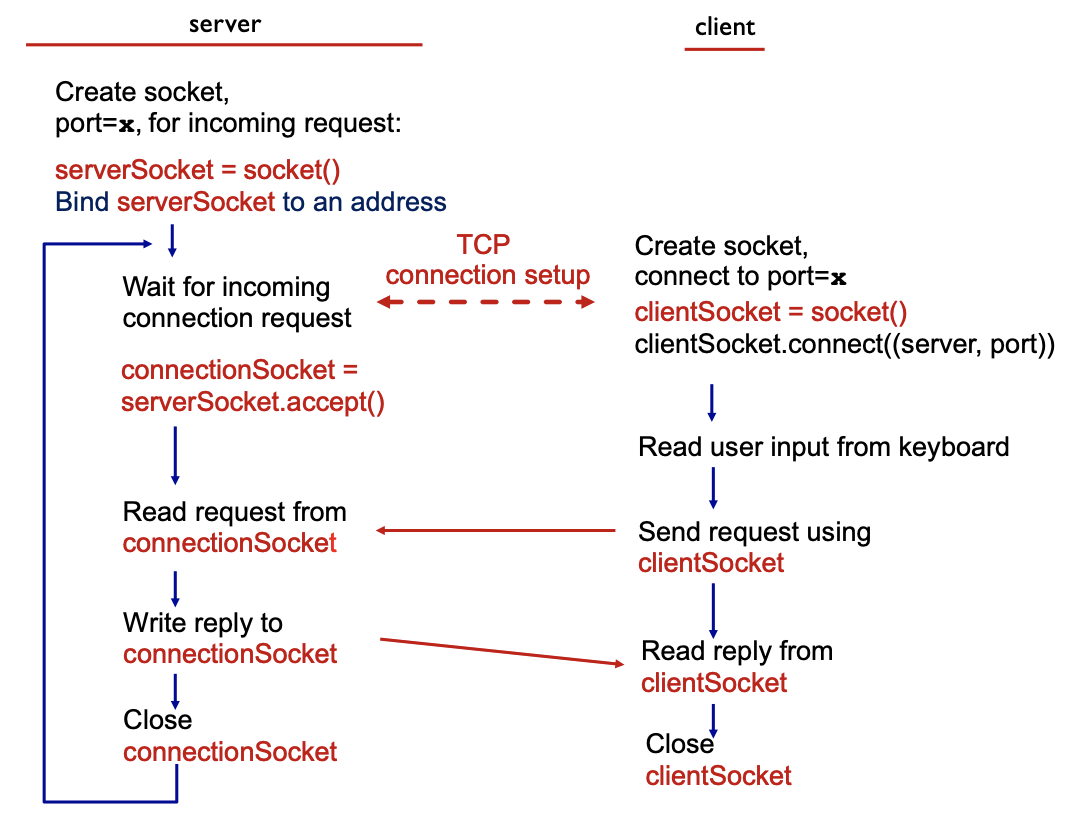
\includegraphics[width=0.6\textwidth]{images/prac-2-1.png}
    \caption{}
    \label{fig:prac-2-1}
\end{figure}
